\subsection{Die Wissenstr�gerschnittstelle}
Bei der Wissenstr�gerschnittstelle handelt es sich um eine Methode zur Datenerfassung, die einen direkten Wissenstransfer zwischen einem Wissenstr�ger und dem Expertensystem erm�glicht. Da die Daten manuell eingegeben und maschinell verarbeitet werden, bezeichnet man die Wissenstr�gerschnittstelle als semi-automatisierte Wissenserfassungsmethode. Im Folgenden werden zwei Anwendungsbeispiele aus unterschiedlichen Bereichen betrachtet und in Bezug auf die wichtigsten Erkenntnisse bei der Entwicklung und dem Einsatz zusammengefasst. \\
Ein Beispiel des Einsatzes der Wissenstr�gerschnittstelle bei einem Elektrotechnikunternehmen wird in \cite{gebus2009} vorgestellt. In der Fallstudie wird ein bereits bestehendes \ac{DSS} untersucht, das die F�hrungskr�fte bei den Entscheidungen von nicht-strukturieren Problemen in der Produktion unterst�tzt \cite[S.94]{gebus2009}. Das Problem dabei besteht darin, dass in der Datenbank des DSS nur die Daten von Produkteigenschaften gesammelt werden. Die Produktionsprozesse werden allerdings von Experten gesteuert, die mithilfe des Erfahrungswissens St�rungen in der Produktion beseitigen. Als Folge hat die Unternehmensf�hrung einen begrenzten �berblick �ber die Situation in der Produktionsabteilung. Au�erdem besteht die Gefahr, dass das spezifische Expertenwissen verloren geht falls der Wissenstr�ger das Unternehmen verl�sst.\\
Die Zielsetzung von \cite{gebus2009} ist das Expertenwissen ins System zu integrieren und dementsprechend ein wissensbasiertes System zu schaffen. Um das Wissen aus der Produktionsabteilung zu erschlie�en, wollen Gebus und Leivisk{\"a} das System um eine Schnittstelle (User Interface) f�r Anlagenbediener erweitern. Als erster Schritt spezifizieren Gebus und Leivisk{\"a} die Nutzergruppen des Systems:
\begin{itemize}
\item Anlagenbediener (Experte), der sein Wissen zu den St�rungen mittels der Wissenstr�gerschnittstelle in die Datenbank eingibt.
\item Administrator, der das gesamte DSS verwaltet und gegebenenfalls die Systemeinstellungen im Hinblick auf die Informationen vom Experten anpasst.
\item Qualit�tsabteilung, die die St�rungsstatistik analysiert, eine Qualit�tsr�ckmeldung an die Produktion und einen Bericht an die F�hrungskraft �bermittelt.
\item F�hrungskraft, die eine umfangreiche �bersicht von der Qualit�tsabteilung erh�lt und davon ausgehend Entscheidungen zur Prozessoptimierung trifft.
\end{itemize}
Jeder Nutzergruppe wird eine geeignete Benutzerschnittstelle zur Verf�gung gestellt. Schematisch l�sst sich die Struktur und die Informationsfl�sse im DSS in der Abbildung \ref{dss_gebus} vereinfacht nachbilden.
\begin{figure}[H] 
	\centering
	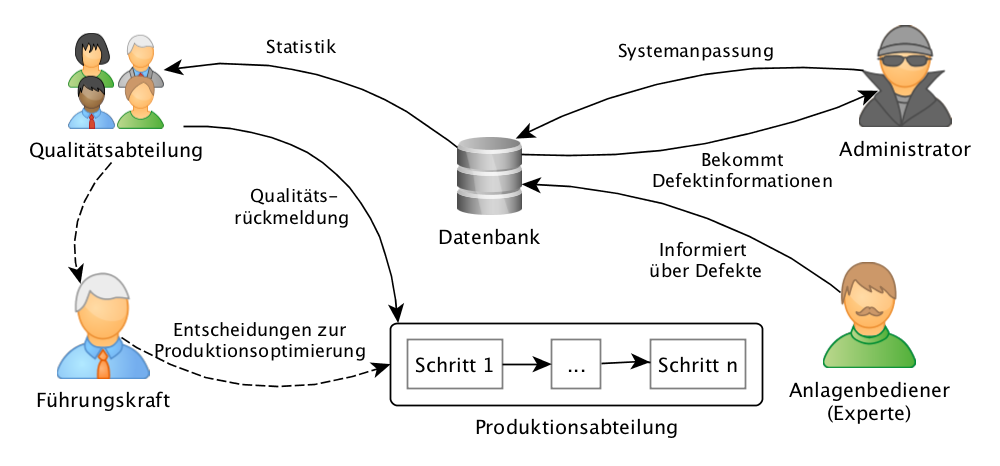
\includegraphics[width=0.9\textwidth]{images/dss_gebus.png}
	\caption{Die Struktur und die Informationsfl�sse im DSS, \cite[S.98]{gebus2009}}
	\label{dss_gebus}
\end{figure} 
%Gem��